
\documentclass[10pt]{article}
%	options include 12pt or 11pt or 10pt
%	classes include article, report, book, letter, thesis

\usepackage[a4paper,bindingoffset=0.2in,%
            left=1in,right=1in,top=0.2in,bottom=0.3in,%
            footskip=.15in]{geometry}
            
\usepackage[T1]{fontenc}
\usepackage[polish]{babel}
\usepackage[utf8]{inputenc}
\usepackage{lmodern}
\selectlanguage{polish}
\usepackage{blindtext}
\usepackage{pgfplots}
\usepackage{graphicx}

\title{Algorytmy numeryczne}
\author{Zadanie 1 \\ Aleksander Kosma\\grupa 1 tester-programista}
\date{13 Październik 2017}

\begin{document}
\maketitle 

\section{Sumowanie szeregów potęgowych}



Niniejsze opracowanie prezentuje badania i wnioski z prób wyliczenia wartości funkcji arctan.
Odnośnikiem w postaci wyniku były wartości funkcji obliczane przez wbudowaną bibliotekę Math.
Wykorzystałem dwa znane mi sposoby na obliczenie tej wartości. Są to:\\
-zsumowanie elementów wyliczonych z szeregu potęgowego:\\
$$arctg(x) = \sum_{n=0}^{\infty}\frac{(-1)^n}{2n + 1} x^{2n + 1}$$
-zsumowanie elementów wyliczonych na podstawie poprzednika:\\
$$a_{n+1}= a *-\frac{x^2 * (2n + 1)}{2n + 3}$$

Ze względu na charakter obliczeń podzieliłem owe zsumowania na kolejne dwa:\\
-zsumowanie elementów licząc od tyłu\\
-zsumowanie elementów licząc od przodu\\

Pracując na zmiennej typu Double zmuszony zostałem do ograniczenia swoich obliczeń do 15-17 miejsc po przecinku.
Pomimo dość niskiej precyzji obliczeń da się zauważyć pewne zachowania w wynikach. Okazuje się, że wyniki
zsumowanych elementów od przodu i od tyłu dają różne rezultaty. Również ze względu na zbieżność szeregu w $[-1,1]$ 
liczyłem tylko dla tego zakresu.

Pierwszy wykres prezentuje procentowe szanse na precyzyjniejszy wynik dla sumowań.
Można zauważyć że bardzo dużą przewagę ma sumowanie od tyłu. Szczególnie w okolicach $[-0.5,0.5]$

\begin{center}
 \makebox[\textwidth]{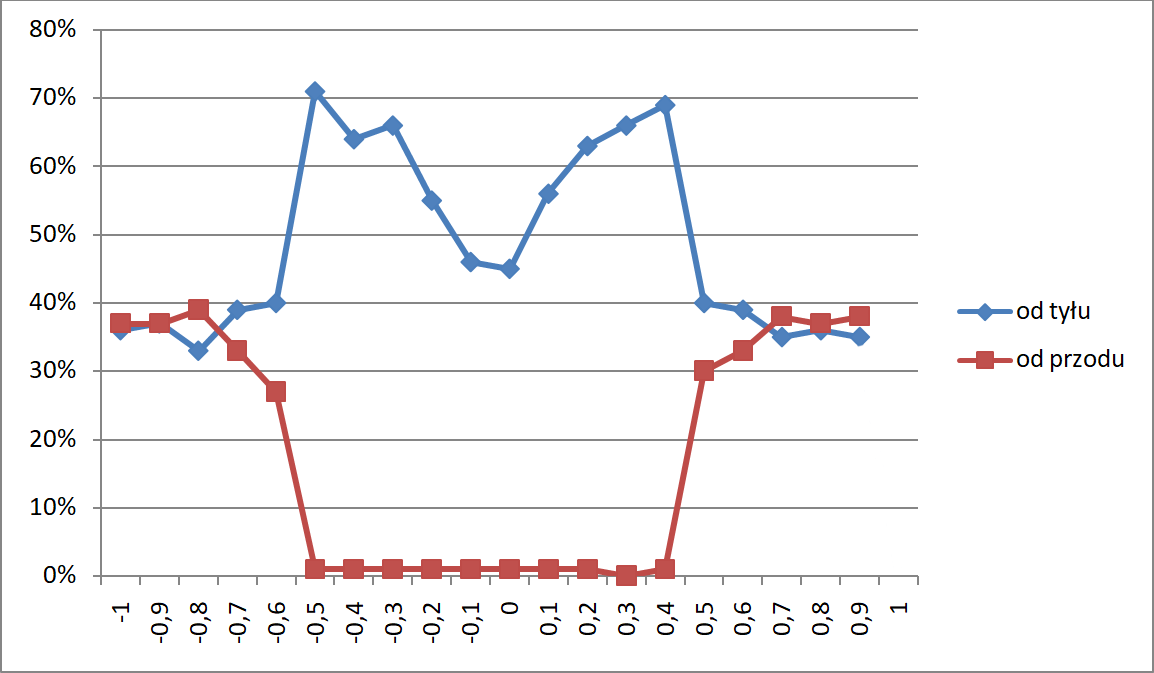
\includegraphics[width=0.55\paperwidth]{rozklad_procentowy.png}}
\end{center}

Drugi wykres prezentuje bezwzględną różnice miedzy wynikiem biblioteki a sumowaniami. 
Środkowa część wykresu ukazuje wyższość sumowania od tyłu. Jest ono precyzyjniejsze nawet o 2 rzędy wielkości.


\begin{center}
 \makebox[\textwidth]{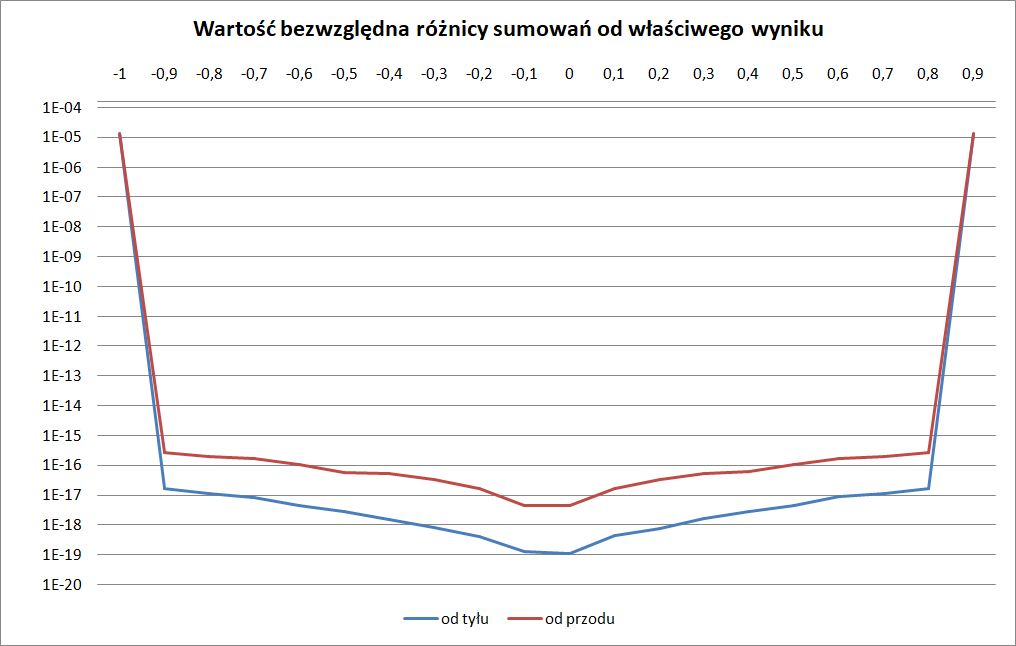
\includegraphics[width=0.65\paperwidth]{rozklad.png}}
\end{center}

Takie rezultaty wynikają z natury działania zmiennej double. W przypadku sumowania liczby większej do liczby mniejszej(gdzie różnica wynosi parę rzędów wielkości), zmienna odrzuca końcowe cyfry mniejszej liczby by pomieścić 
najistotniejsze wartości. Stąd utrata precyzji. W momencie kiedy dwie liczby mają podobną wartość, ich suma potrzebować będzie podobnej precyzji do zapisania wyniku. W konsekwencji nie odrzuci danych. Podsumowując kwestie precyzji wyniku. Opierając się o zmienną double, można stwierdzić, że precyzja wyniku waha się między  14 ,a 16 miejscem po przecinku.\\
Na obrazku poniżej znajduje przy praktyczny przykład. Dla uproszczenia zagadnienia jest on prezentowany na zmiennej float(32 bity) która zazwyczaj mieści w sobie 8 cyfr dziesiętnych.


\begin{center}
 \makebox[\textwidth]{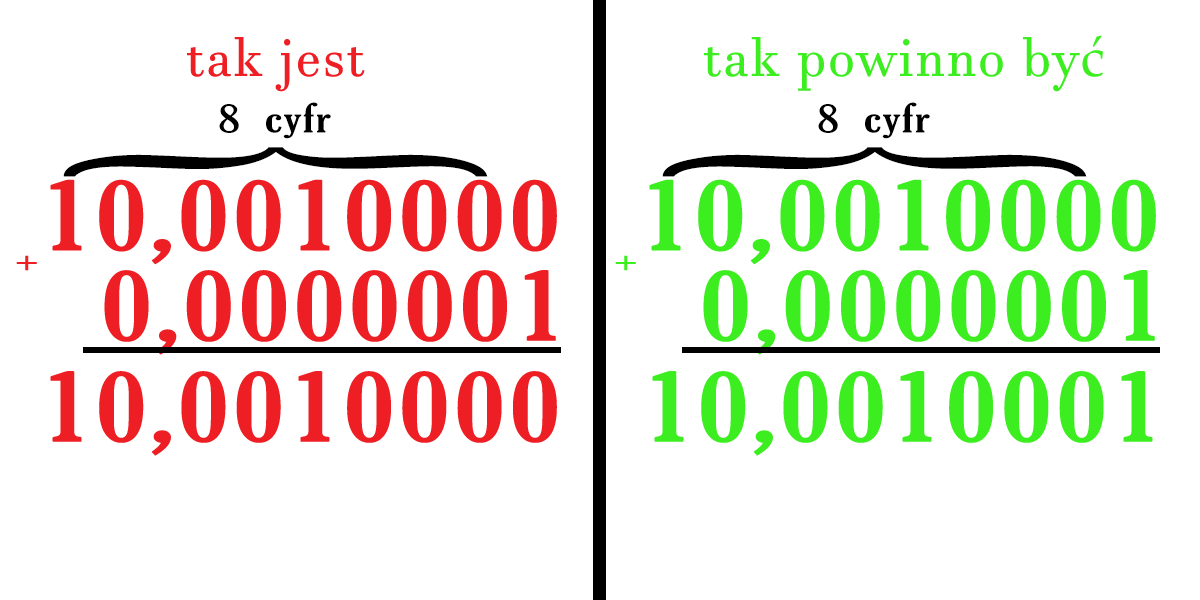
\includegraphics[width=0.4\paperwidth]{przyklad.png}}
\end{center}
By rozwiązać problem niskiej precyzji, który zaistniał w przypadku doubla, trzeba mieć kontrolę nad precyzją obliczeń. Rozwiązaniem może okazać się klasa BigDecimal. Klasa ta może przechować nieograniczoną 
wartość liczbową, ogranicza ją jedynie skala która osiąga wartość 32-bitowego integera, czyli trochę 
ponad dwa miliardy miejsc. \\
Niestety nie udało mi się osiagnąć zamierzonej precyzji. W okolicach 17-19 miejsca wynik na BigDeciamalu zaczyna różnić się na tle wyniku z Wolfram(computational knowledge engine). Wzór wydaje się jak najbardziej dobry, więc obwiniam obliczenia lub konwersje które dzieją się może na doublach do których nie mam dostępu lub o nich nie wiem.\\

Zdarzały się sytuacje, w których przybliżenie wyniku biblioteki różniło się od wyniku z Woflram. Za to wynik na BigDecimalach był precyzyjniejszy. Niestety ze względu na brak szybkiego dostępu do wyników z wolfram z poziomu kodu ciężko stworzyć realne statystyki. Oto tylko parę przykładów z moich obliczeń, lecz one nic nie dowodzą:

\begin{center}
 \makebox[\textwidth]{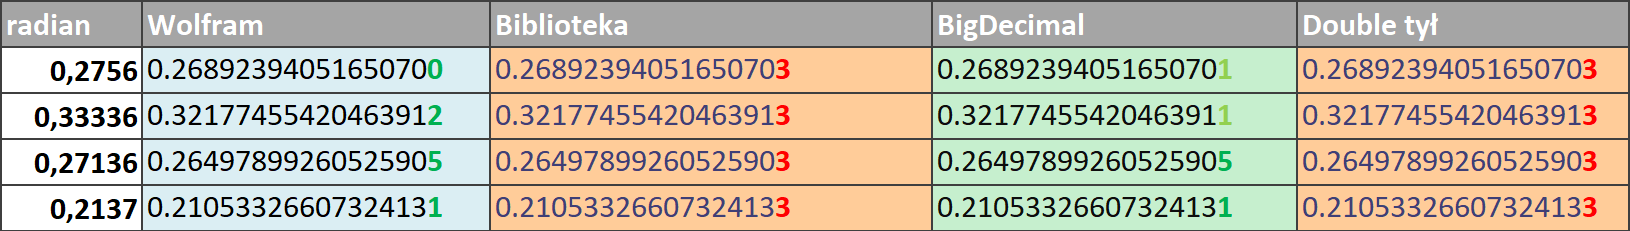
\includegraphics[width=0.75\paperwidth]{bigDecimal.png}}
\end{center}








Dane do wykresów o doublach obliczone zostały na 2 milionach próbek.

\end{document}